\documentclass[11pt]{article}
\usepackage[margin=1in]{geometry}
\usepackage{amsmath,amssymb,mathtools,bm}
\usepackage{graphicx}
\usepackage{booktabs,array}
\usepackage{enumitem}
\usepackage{xcolor}
\usepackage{hyperref}
\usepackage{float}
\hypersetup{
    colorlinks=true,
    linkcolor=blue,
    urlcolor=blue,
    pdftitle={OLS in Matrix Form: Study Notes},
    pdfauthor={OLS in Matrix Form}
}
\setlist[itemize]{topsep=3pt,itemsep=2pt}
\setlist[enumerate]{topsep=3pt,itemsep=2pt}
\newcommand{\bhat}{\hat{\boldsymbol{\beta}}}
\newcommand{\eps}{\boldsymbol{\varepsilon}}
\newcommand{\ee}{\mathbf{e}}
\newcommand{\XX}{\mathbf{X}}
\newcommand{\yy}{\mathbf{y}}
\newcommand{\RSS}{\operatorname{RSS}}

\begin{document}

\begin{titlepage}
    \centering
    \vspace*{\fill}
    {\Huge\bfseries OLS in Matrix Form\par}
    \vspace{1.5em}
    {\Large Noted by Md. Inzamamul Lohani\\
Software Engineering, IIT, DU\par}
    \vspace{2em}
    {\large 17 November 2026\par}
    \vspace*{\fill}
\end{titlepage}
\setcounter{page}{2}

\tableofcontents
\newpage

\section{The True Model}

The population regression model in matrix notation is
\begin{equation}
    \boxed{\yy=\XX\boldsymbol{\beta}+\eps.}
    \label{eq:true-model}
\end{equation}
Here:
\begin{itemize}
    \item $\XX$ is an $n\times k$ matrix containing observations on $k$ independent variables for $n$ observations. If the model includes a constant (intercept), one column of $\XX$ consists entirely of ones.
    \item $\yy$ is an $n\times 1$ vector of observations on the dependent variable.
    \item $\eps$ is an $n\times 1$ vector of disturbances (unobserved influences).
    \item $\boldsymbol{\beta}$ is a $k\times 1$ vector of unknown population parameters.
\end{itemize}
The model has a \textbf{systematic component}, $\XX\boldsymbol{\beta}$, and a \textbf{stochastic component}, $\eps$. The objective is to estimate the unknown population parameters in $\boldsymbol{\beta}$.

\subsection{Dimensions}
The dimensions are chosen so that the matrix multiplication is valid:
\[
(n\times k)(k\times 1)=n\times 1.
\]
Thus $\XX\boldsymbol{\beta}$ has the same dimension as $\yy$ and $\eps$.

\begin{figure}[H]
\centering
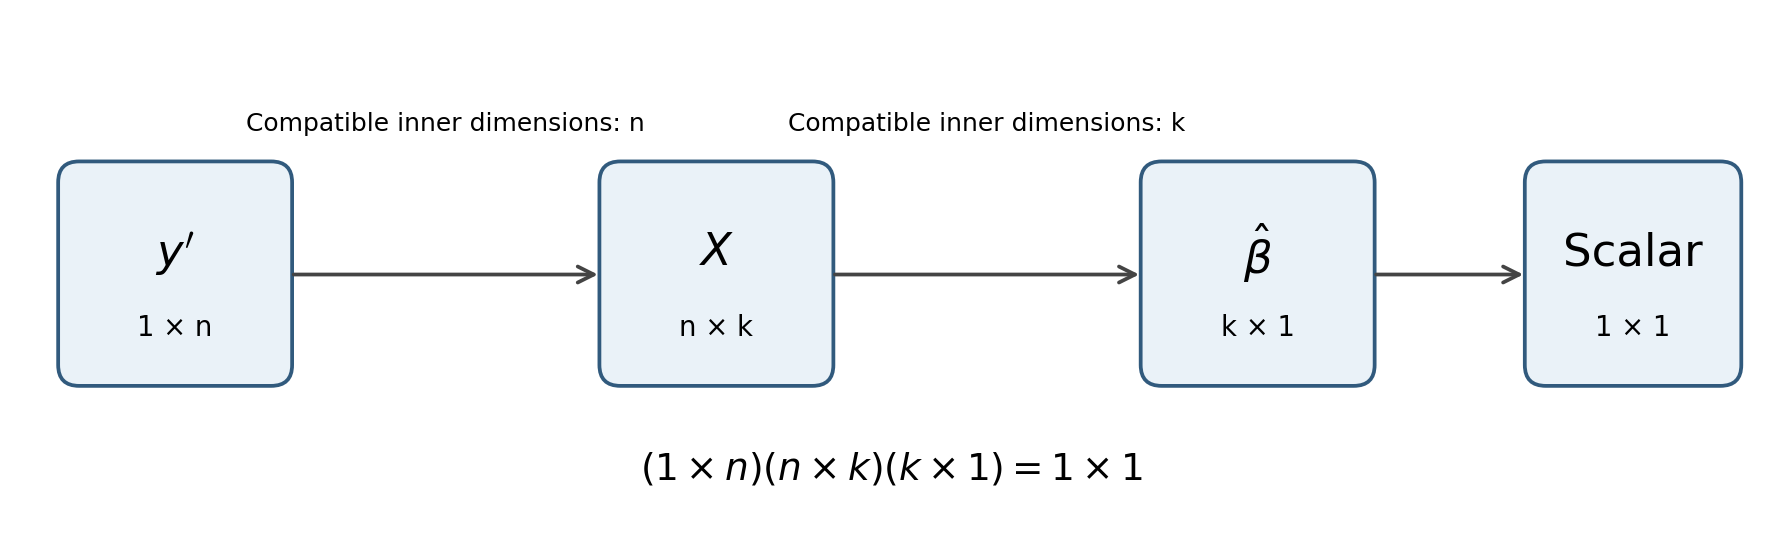
\includegraphics[width=0.92\textwidth]{images/matrix_dimensions.png}
\caption{Dimension check for the scalar product $\yy'\XX\bhat$.}
\end{figure}

\section{Estimates, Fitted Values, and Residuals}

The estimated parameter vector is denoted by $\bhat$. The fitted (predicted) values are
\[
\widehat{\yy}=\XX\bhat.
\]
The residual vector is the difference between observed and fitted values:
\begin{equation}
    \boxed{\ee=\yy-\XX\bhat.}
    \label{eq:residual}
\end{equation}
A residual is observable because it can be calculated from the sample.

\subsection{Disturbances versus residuals}
These terms must be distinguished:
\begin{center}
\begin{tabular}{p{0.18\textwidth}p{0.34\textwidth}p{0.34\textwidth}}
\toprule
 & \textbf{Disturbance $\eps$} & \textbf{Residual $\ee$}\\
\midrule
Meaning & Unobserved part of the population model & Observed minus fitted value\\
Observable? & No & Yes\\
Role & Part of the true model & Computed after estimating the model\\
\bottomrule
\end{tabular}
\end{center}
In general, $\eps\ne\ee$. Do not infer properties of the unobserved disturbances merely from properties of the residuals.

\section{The OLS Criterion: Minimize the Sum of Squared Residuals}

The sum of squared residuals (RSS) is
\begin{equation}
    \RSS=\ee'\ee.
\end{equation}
Since $\ee=\yy-\XX\bhat$,
\begin{equation}
    \RSS=(\yy-\XX\bhat)'(\yy-\XX\bhat).
    \label{eq:rss-start}
\end{equation}
The transpose of a product reverses the order:
\[
(AB)'=B'A',
\qquad
(A-B)'=A'-B'.
\]
Therefore,
\[
(\yy-\XX\bhat)'=\yy'-(\XX\bhat)'=\yy'-\bhat'\XX'.
\]
Substituting into \eqref{eq:rss-start} gives
\begin{align}
\RSS
&=(\yy'-\bhat'\XX')(\yy-\XX\bhat)\\
&=\yy'\yy-\yy'\XX\bhat-\bhat'\XX'\yy+\bhat'\XX'\XX\bhat.
\end{align}
The middle expressions are scalars. A scalar is equal to its transpose, so
\[
\yy'\XX\bhat=(\yy'\XX\bhat)'=\bhat'\XX'\yy.
\]
Hence the two middle terms are equal, and
\begin{equation}
    \boxed{\RSS=\yy'\yy-2\bhat'\XX'\yy+\bhat'\XX'\XX\bhat.}
    \label{eq:rss-expanded}
\end{equation}

\subsection{Why is $\yy'\XX\bhat$ a scalar?}
The dimensions are
\[
\underbrace{\yy'}_{1\times n}
\underbrace{\XX}_{n\times k}
\underbrace{\bhat}_{k\times 1}.
\]
Multiplying from left to right,
\[
(1\times n)(n\times k)=1\times k,
\qquad
(1\times k)(k\times 1)=1\times 1.
\]
A $1\times 1$ matrix contains one number, so it is a scalar.

\begin{figure}[H]
\centering
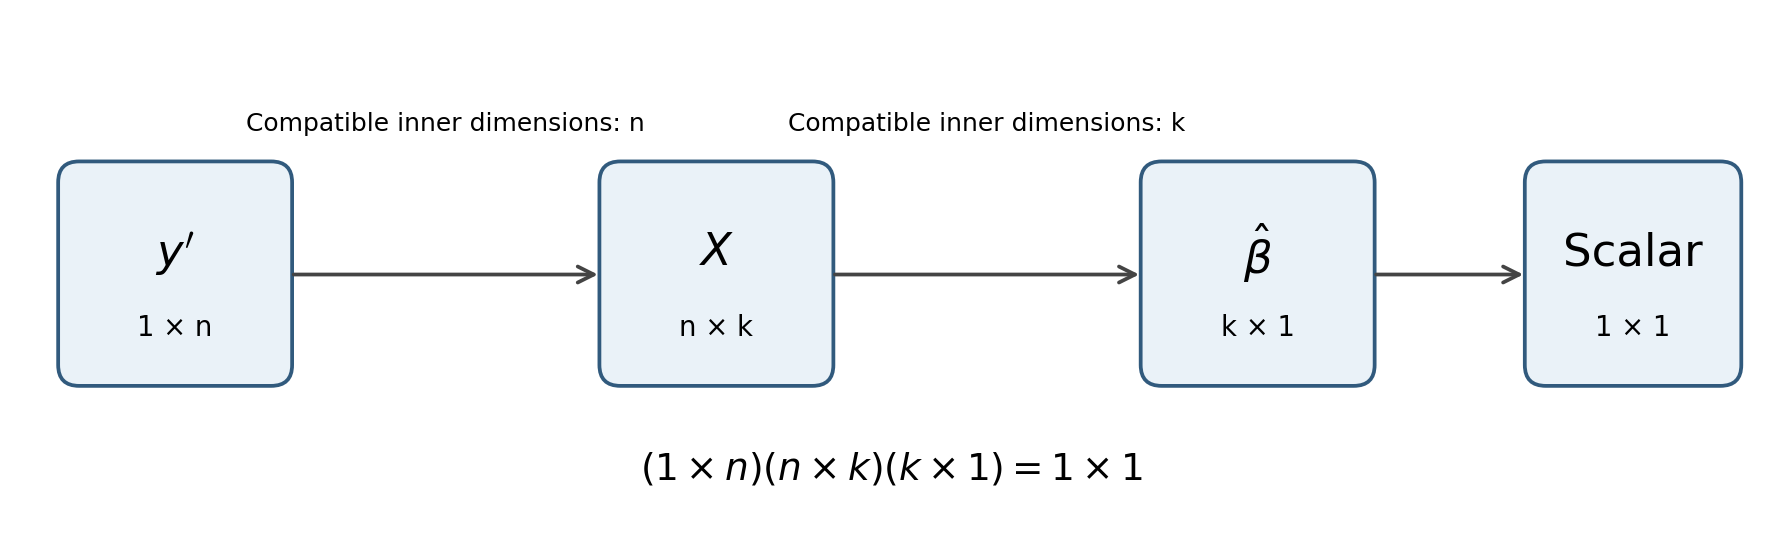
\includegraphics[width=0.92\textwidth]{images/matrix_dimensions.png}
\caption{The final dimension of $\yy'\XX\bhat$ is $1\times 1$.}
\end{figure}

\section{Differentiating RSS with Respect to the Coefficient Vector}

We choose $\bhat$ to minimize RSS. Differentiate each term in \eqref{eq:rss-expanded} with respect to the vector $\bhat$.

\subsection{Useful matrix differentiation rules}
For vectors $\mathbf{a}$ and $\mathbf{b}$ of compatible dimensions,
\[
\frac{\partial(\mathbf{b}'\mathbf{a})}{\partial\mathbf{b}}=\mathbf{a}.
\]
For a square matrix $A$,
\begin{equation}
    \frac{\partial(\boldsymbol{\beta}'A\boldsymbol{\beta})}
    {\partial\boldsymbol{\beta}}
    =(A+A')\boldsymbol{\beta}.
    \label{eq:quadratic-rule}
\end{equation}
If $A$ is symmetric ($A'=A$), this becomes
\[
\frac{\partial(\boldsymbol{\beta}'A\boldsymbol{\beta})}
{\partial\boldsymbol{\beta}}=2A\boldsymbol{\beta}.
\]

\subsection{Deriving the quadratic-form rule}
Let $f(\boldsymbol{\beta})=\boldsymbol{\beta}'A\boldsymbol{\beta}$. Using the product rule in differential form,
\[
df=d\boldsymbol{\beta}'A\boldsymbol{\beta}
+\boldsymbol{\beta}'A\,d\boldsymbol{\beta}.
\]
The second term is a scalar, so it equals its transpose:
\[
\boldsymbol{\beta}'A\,d\boldsymbol{\beta}
=(\boldsymbol{\beta}'A\,d\boldsymbol{\beta})'
=d\boldsymbol{\beta}'A'\boldsymbol{\beta}.
\]
Thus
\[
df=d\boldsymbol{\beta}'A\boldsymbol{\beta}
+d\boldsymbol{\beta}'A'\boldsymbol{\beta}
=d\boldsymbol{\beta}'(A+A')\boldsymbol{\beta}.
\]
Therefore the gradient is $(A+A')\boldsymbol{\beta}$, proving \eqref{eq:quadratic-rule}.

\subsection{Differentiate the three RSS terms}
Starting from
\[
\RSS=\underbrace{\yy'\yy}_{\text{Term 1}}
-\underbrace{2\bhat'\XX'\yy}_{\text{Term 2}}
+\underbrace{\bhat'\XX'\XX\bhat}_{\text{Term 3}},
\]
we obtain:
\begin{align*}
\frac{\partial(\yy'\yy)}{\partial\bhat}&=0,
&&\text{because $\yy$ is fixed with respect to $\bhat$},\\
\frac{\partial(-2\bhat'\XX'\yy)}{\partial\bhat}&=-2\XX'\yy,\\
\frac{\partial(\bhat'\XX'\XX\bhat)}{\partial\bhat}
&=\bigl(\XX'\XX+(\XX'\XX)'\bigr)\bhat\\
&=2\XX'\XX\bhat,
&&\text{because $\XX'\XX$ is symmetric.}
\end{align*}
Combining the three derivatives gives
\begin{equation}
    \boxed{\frac{\partial\RSS}{\partial\bhat}
    =-2\XX'\yy+2\XX'\XX\bhat.}
    \label{eq:rss-gradient}
\end{equation}

\section{Normal Equations and the OLS Estimator}

At an interior minimum, the first derivative (gradient) is zero:
\[
-2\XX'\yy+2\XX'\XX\bhat=0.
\]
Divide by $2$ and rearrange:
\begin{equation}
    \boxed{\XX'\XX\bhat=\XX'\yy.}
    \label{eq:normal}
\end{equation}
These are the \textbf{normal equations}.

The matrix $\XX'\XX$ is $k\times k$, square, and symmetric. If it is invertible, pre-multiply both sides of \eqref{eq:normal} by $(\XX'\XX)^{-1}$:
\[
(\XX'\XX)^{-1}\XX'\XX\bhat=(\XX'\XX)^{-1}\XX'\yy.
\]
Since $(\XX'\XX)^{-1}\XX'\XX=I_k$,
\begin{equation}
    \boxed{\bhat=(\XX'\XX)^{-1}\XX'\yy.}
    \label{eq:ols-estimator}
\end{equation}
This is the OLS estimator in matrix form.

\subsection{When might the inverse fail to exist?}
The inverse of $\XX'\XX$ may not exist if:
\begin{itemize}
    \item $n<k$, so there are fewer observations than independent variables; or
    \item there is perfect multicollinearity, meaning one or more columns of $\XX$ are exact linear combinations of other columns.
\end{itemize}
The full-rank condition rules out these cases.

\section{Checking That the Stationary Point Is a Minimum}

Differentiate the gradient in \eqref{eq:rss-gradient} again with respect to $\bhat$. The Hessian matrix is
\[
\frac{\partial^2\RSS}{\partial\bhat\,\partial\bhat'}
=2\XX'\XX.
\]
If $\XX$ has full column rank, then $\XX'\XX$ is positive definite. Therefore the Hessian is positive definite, and the stationary point is a minimum.

\section{A Fundamental OLS Property: $\XX'\ee=0$}

Start with the normal equations:
\[
\XX'\XX\bhat=\XX'\yy.
\]
Using $\ee=\yy-\XX\bhat$,
\begin{align*}
\XX'\ee
&=\XX'(\yy-\XX\bhat)\\
&=\XX'\yy-\XX'\XX\bhat\\
&=\XX'\yy-\XX'\yy\\
&=\mathbf{0}.
\end{align*}
Therefore,
\begin{equation}
    \boxed{\XX'\ee=\mathbf{0}.}
    \label{eq:xte}
\end{equation}
This says that the residual vector is orthogonal to every column of the regressor matrix.

\begin{figure}[H]
\centering
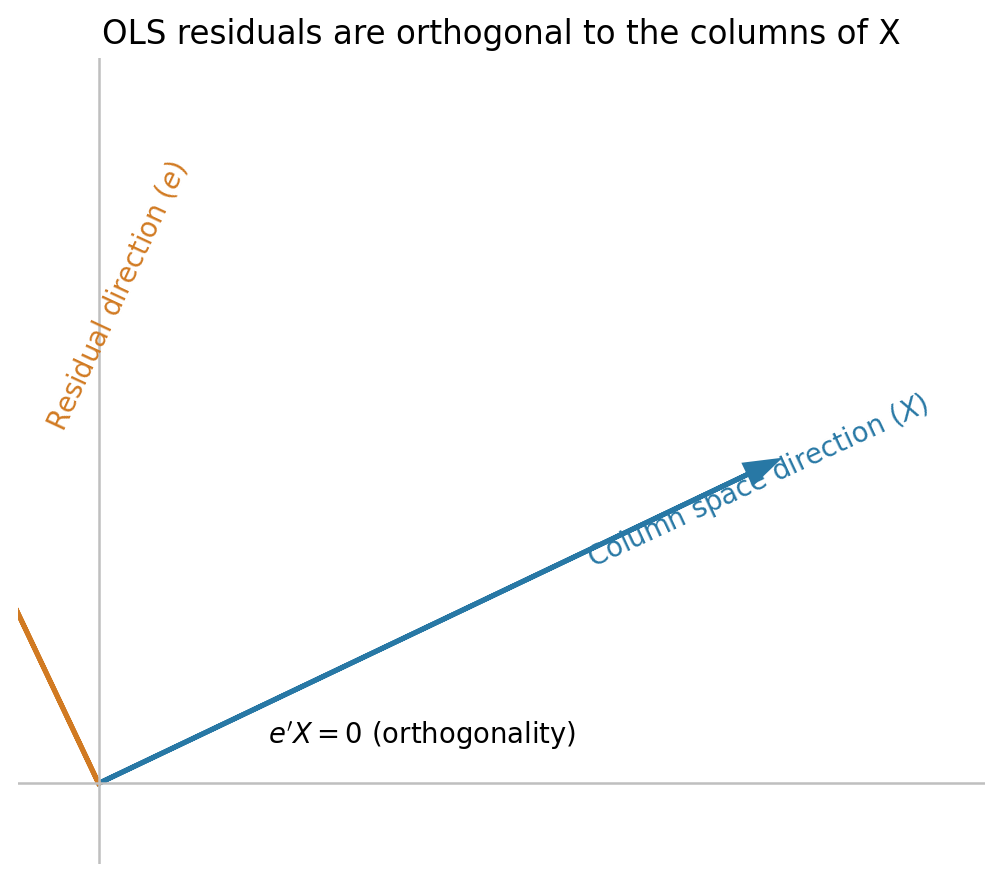
\includegraphics[width=0.70\textwidth]{images/residual_orthogonality.png}
\caption{Conceptual illustration of residual orthogonality. The residual direction is perpendicular to the column-space direction.}
\end{figure}

\subsection{Column-by-column interpretation}
If $\mathbf{x}_j$ is the $j$th column of $\XX$, then \eqref{eq:xte} implies
\[
\mathbf{x}_j'\ee=0
\qquad \text{for every }j=1,\ldots,k.
\]
In sample terms, each regressor has zero sample inner product with the residual vector. With the usual intercept specification, this also corresponds to zero sample covariance/correlation between each regressor and the residuals (provided the relevant variances are nonzero).

This is a property of the \textbf{observed regressors and residuals}. It does not by itself establish that regressors are uncorrelated with the unobserved disturbances.

\section{Consequences When the Model Includes a Constant}

If the regression includes an intercept, one column of $\XX$ is a vector of ones:
\[
\mathbf{1}=
\begin{bmatrix}1&1&\cdots&1\end{bmatrix}'.
\]
The corresponding element of $\XX'\ee=\mathbf{0}$ is
\[
\mathbf{1}'\ee=0.
\]
Therefore,
\begin{equation}
    \boxed{\sum_{i=1}^{n}e_i=0.}
\end{equation}
The sample mean of the residuals is consequently
\[
\boxed{\bar e=\frac{1}{n}\sum_{i=1}^{n}e_i=0.}
\]
These two properties require an intercept in the regression.

\section{Key Ideas at a Glance}

\begin{center}
\begin{tabular}{p{0.29\textwidth}p{0.61\textwidth}}
\toprule
\textbf{Concept} & \textbf{Main result}\\
\midrule
True model & $\yy=\XX\boldsymbol{\beta}+\eps$\\
Fitted values & $\widehat{\yy}=\XX\bhat$\\
Residuals & $\ee=\yy-\XX\bhat$\\
RSS & $\RSS=\ee'\ee$\\
Expanded RSS & $\yy'\yy-2\bhat'\XX'\yy+\bhat'\XX'\XX\bhat$\\
RSS gradient & $-2\XX'\yy+2\XX'\XX\bhat$\\
Normal equations & $\XX'\XX\bhat=\XX'\yy$\\
OLS estimator & $\bhat=(\XX'\XX)^{-1}\XX'\yy$\\
Residual orthogonality & $\XX'\ee=\mathbf{0}$\\
With an intercept & $\sum_i e_i=0$ and $\bar e=0$\\
\bottomrule
\end{tabular}
\end{center}

\section{Practice Questions}

\begin{enumerate}
    \item If $\XX$ is $n\times k$, what are the dimensions of $\XX'$, $\XX'\XX$, and $\XX'\yy$?
    \item Why is $\yy'\XX\bhat$ a scalar?
    \item Explain why $\yy'\XX\bhat=\bhat'\XX'\yy$.
    \item Expand $(\yy-\XX\bhat)'(\yy-\XX\bhat)$ step by step.
    \item Why does the derivative of $\yy'\yy$ with respect to $\bhat$ equal zero?
    \item State the derivative of $\boldsymbol{\beta}'A\boldsymbol{\beta}$ when $A$ is symmetric.
    \item Derive the normal equations from the RSS gradient.
    \item Under what condition can the OLS estimator be written using $(\XX'\XX)^{-1}$?
    \item Derive $\XX'\ee=\mathbf{0}$ from the normal equations.
    \item Why does including a constant imply that the residuals sum to zero?
\end{enumerate}

\section*{Scope of These Notes}
\addcontentsline{toc}{section}{Scope of These Notes}
These notes cover the material discussed so far from the supplied document: the true model, estimates and residuals, the RSS criterion, its matrix expansion and differentiation, the normal equations, the OLS estimator, the minimum check, and the first residual properties. Later sections of the source document (Gauss--Markov assumptions and theorem, variance-covariance matrix, robust standard errors, partitioned regression, and the Frisch--Waugh--Lovell theorem) are not included in this installment.

\end{document}
